\documentclass[a4paper,11pt,reqno]{amsart}
\usepackage{M67tds}

\newlist{axioms}{description}{1}
\newcommand\axiomlabel[1]{\hfill\textbf{(#1)}}
\setlist[axioms]{style=nextline,before={\let\makelabel\axiomlabel}}
\newcommand*{\ensemble}[3][]{#1\{ #2 \;#1|\; #3 #1\}} % par exemple \ensemble[\big]{x^2}{x \in \R}

\begin{document}

\hautdepage{TD2: Géométrie plane}

\begin{convention}
  On se place dans le plan $\ens{P}=\R^2$.
\end{convention}


% ==================================
\section{Axiomatique}
% ==================================

On rappelle les propriétés d'incidence et d'ordre:\\[-1.7\baselineskip]
\begin{multicols}{2}\small
  \begin{axioms}[leftmargin=3.5em]
    \item[I1] par deux points distincts passe une unique droite,
    \item[I2] toute droite contient au moins deux points distincts,
    \item[I3] il existe trois points non alignés,
    \item[O1] si $C$ est entre $A$ et $B$, alors $A$, $B$ et $C$ sont alignés, deux à deux distincts et $C$ est aussi entre $B$ et $A$,
    \item[O2] pour tous points distincts $A$ et $B$ il existe un point $C$ tel que $B$ soit entre $A$ et $C$,
    \item[O3] parmi trois points alignés deux à deux distincts, un et un seul d'entre eux est entre les deux autres,
    \item[O4] soient $A$, $B$, et $C$ trois points non alignés et $\ens{D}$ une droite ne passant par aucun d'eux. Si $\ens{D}$ passe par un point $D$ entre $A$ et $B$, alors $\ens{D}$ passe ou bien par un point entre $A$ et $C$, ou bien par un point entre $B$ et $C$, mais pas les deux à la fois.
  \end{axioms}
\end{multicols}\vspace{7pt}

%-----------------------------------
\begin{exo}

  En utilisant seulement les propriétés d'incidence et d'ordre, montrer que
  \begin{enumerate}
    \item toute droite possède une infinité de points;
    \item par tout point passent une infinité de droites;
    \item entre deux points distincts $A$ et $B$ il existe toujours un point $C$.
  \end{enumerate}
\end{exo}

%-----------------------------------
\begin{exo}

  Trouver un ensemble fini possédant une géométrie vérifiant les trois propriétés d'incidence \textbf{(I1-3)}, c.-à-d. un ensemble muni de sous-ensembles appelés \emph{droites} vérifiant les propriétés d'incidence.\\
  Existe-t-il un ensemble fini possédant une géométrie vérifiant les sept propriétés \textbf{I1-O4} ?
\end{exo}

%-----------------------------------
\begin{exo} (Extrait du DS1 de 2018)
  \sidebyside{.7}{
    En utilisant seulement les propriétés \textbf{I1} à \textbf{O4} démontrer que si deux points distincts $C$ et $D$ sont entre $A$ et $B$ alors soit $D$ est entre $A$ et $C$,  soit $D$ est entre $B$ et $C$.\\
    \begin{indication}
      Vous pouvez vous inspirer du dessin ci-contre.
    \end{indication}
  }{
      \raisebox{-28mm}[0pt][0pt]{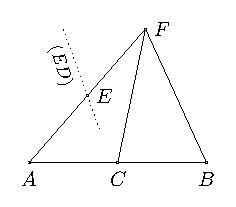
\includegraphics[width=5cm]{M67_2017-18_DS1_img_ordre}}
  }
\end{exo}

%-----------------------------------
\begin{exo}[.7] (Barycentre)

  Soient deux points $A \neq B$. Montrer que les assertions suivantes sont équivalentes.\\[-1.7\baselineskip]
  \begin{multicols}{2}
    \begin{enumerate}
      \item $M \in (AB)$;
      \item $\exists! \lambda \in \mathbb{R}, M=(1-\lambda) A + \lambda B $;
      \item $\exists! \mu  \in \mathbb{R}, M=\mu A + (1-\mu) B $;
      \item $\exists! s,t  \in \mathbb{R}, s+t=1, M=s A + t B $;
    \end{enumerate}
  \end{multicols}
\end{exo}

%-----------------------------------
\begin{exo} (Extrémités d'un segment, origine d'une demi-droite)

  \begin{enumerate}
    \item Soient $A$ et $B$ deux points du plan. On rappelle que si $A \neq B$ les points \emph{entre} $A$ et $B$ sont les points de la forme $\lambda A + (1-\lambda) B$ avec $\lambda \in ]0,1[$, que leur ensemble est noté $]AB[$, et que le segment $[AB]$ est défini comme l'ensemble contenant $A$, $B$ et tous les points entre $A$ et $B$. Dans le cas où $A=B$, nous avons $]AB[ = \emptyset$ et $[AB] = \left\{ A \right\}$.
    \begin{enumerate}
      \item Montrer qu'il n'existe aucuns points $C$ et $D$ appartenant à $[AB]$ tels que $A$ soit entre $C$ et $D$.
      \item En déduire que le couple non ordonné $\{A,B\}$ est déterminé par le segment $[AB]$.
    \end{enumerate}
    \item Pour $A \neq B$ la demi-droite (fermée) $[AB)$ est définie comme l'ensemble des points $M \in (AB)$ tels que $A \notin ]MB[$.
    \begin{enumerate}
      \item Montrer que $[AB) = \ensemble[\big]{(1- \lambda )A + \lambda B}{\lambda \in \R_{+}}$.
      \item Montrer que la demi-droite opposée $\ensemble[\big]{(1- \lambda )A + \lambda B}{\lambda \in \R_{-}}$ est l'image de $[AB)$ par la symétrie centrale de centre $A$.
      \item Montrer que les angles opposés déterminés par deux droites sécantes sont égaux.
      \item Montrer que l'origine $A$ d'une demi-droite $[AB)$ est déterminée par la demi-droite.
    \end{enumerate}
  \end{enumerate}
\end{exo}

%-----------------------------------
\begin{exo} (Propriétés de congruences pour les segments)

On dit que deux segments sont \emph{congruents} s'ils ont la même longueur. On note alors $[AB]\simeq[CD]$ (ou $AB \simeq CD$). Vérifier que nous avons les propriétés (de congruence) suivantes:
  \begin{axioms}[leftmargin=2.8em]
    \item[C1] pour tout segment $[AB]$ et toute demi-droite $[CD)$, il existe un unique point $E$ sur $[CD)$ tel que $[CE]\simeq[AB]$,
    \item[C2] si $[AB]\simeq[CD]$ et $[AB]\simeq[EF]$, alors $[CD]\simeq[EF]$; tout segment est congruent avec lui-même,
    \item[C3] soient $A$, $B$ et $C$ trois points alignés dans cet ordre et $D$, $E$ et $F$ trois autres points alignés dans cet ordre tels que $[AB]\simeq [DE]$ et $[BC]\simeq[EF]$. Alors $[AC]\simeq[DF]$.
  \end{axioms}
\end{exo}


\newpage
% ==================================
\section{Triplets pythagoriciens}
% ==================================

%-----------------------------------
\begin{exo}\label{cerclerat} (Paramétrisation rationnelle du cercle)

  Soit $\ens{C}$ le cercle unité dans le plan, c.-à-d. le cercle de centre $O=(0,0)$ et de rayon $1$. Soient $P$ le point $(-1,0)$ et $\ens{D}$ la droite d'équation $x=0$.
  \begin{enumerate}
    \item Montrer que pour tout point $M \in \ens{D}$ la droite $(PM)$ recoupe $\ens{C}$ en exactement un point $Q \neq P$.
    \item Montrer que l'application $M \mapsto Q$ est une bijection de $\ens{D}$ sur $\ens{C}^\ast=\ens{C} \setminus \{P\}$.
    \item En déduire que $\rho \colon t \longmapsto \left( \dfrac{1-t^2}{1+t^2}, \dfrac{2t}{1+t^2}\right)$ établit une bijection de $\R$ sur $\ens{C}^\ast$. En donner la réciproque.
  \end{enumerate}
  \begin{convention}
      On dit que $\rho$ est une \emph{paramétrisation rationnelle} du cercle $\ens{C}$: c'est une application qui atteint presque tous les points du cercle et dont les coordonnées sont des fractions rationnelles en la variable $t$.
  \end{convention}
  \begin{enumerate}[resume]
    \item Montrer que $\rho(t) \in \Q^2$ si et seulement si $t \in \Q$.
    \item Soit $Q$ un point de $\ens{C}$ distinct de $P$. Quelles sont les coordonnées du point d'intersection de la droite $(PQ)$ et de la droite d'équation $x=1$?
    \item En utilisant la paramétrisation habituelle du cercle $\theta \in \R \mapsto (\cos \theta,\sin \theta)$, retrouver l'expression de $\rho$ (on pourra interpréter $t$ comme une certaine ligne trigonométrique reconnaître une formule connue).
  \end{enumerate}
\end{exo}

%-----------------------------------
\begin{exo} (Triplets pythagoriciens)

  On cherche tous les triangles rectangles dont les côtés sont de longueur entière.
  \begin{enumerate}
    \item Montrer que cela revient à résoudre dans $\Z^3$ l'équation $a^2+b^2=c^2$.
    \item Soit $(a,b,c)$ une solution non nulle. Montrer, en utilisant l'exercice \ref{cerclerat}, qu'il  existe $t \in \Q$ tel que $\dfrac{a}{c}= \dfrac{1-t^2}{1+t^2}$\; et\; $\dfrac{b}{c}= \dfrac{2t}{1+t^2}$.
    \item En déduire qu'un triangle rectangle a tous ses côtés de longueur entière si et seulement si ses côtés sont de longueurs $2kuv$, $k(v^2-u^2)$ et $k(v^2+u^2)$ pour trois entiers non nuls $u$, $v$ et $k$ avec $v>u$.
  \end{enumerate}
\end{exo}


% ==================================
\section{Isométries du plan}
% ==================================

\begin{convention}
  Une isométrie du plan est une application du plan qui préserve les distances, c.-à-d. $f \colon \ens{P} \to \ens{P}$ telle que $f(A)f(B)=AB$ pour tous points $A$ et $B$.
\end{convention}

%-----------------------------------
\begin{exo} (Propriétés des isométries)

\begin{enumerate}
  \item Montrer qu'une isométrie est injective.
  \item Montrer qu'une isométrie $f$ conserve l'alignement et l'ordre sur les droites (plus précisément, les points $A$, $B$ et $C$ sont alignés dans cet ordre si et seulement si leurs images $f(A)$, $f(B)$ et $f(C)$ le sont).
  \item Montrer qu'une isométrie $f$ présèvre les barycentres, c.-à-d. $f\big((1- \lambda )A + \lambda B\big) = (1- \lambda )f(A) + \lambda f(B)$ pour tout deux points $A$ et $B$, et $\lambda \in \mathbb{R}$.
  \item Montrer qu'une isométrie est surjective. En déduire que les isométries forment un groupe.
  \item Montrer qu'une isométrie conserve le parallélisme et l'orthogonalité des droites.
\end{enumerate}
\end{exo}

%-----------------------------------
\begin{exo} (Générateurs du groupe des isométries)

  On montre ici que le groupe des isométries du plan est engendré par les réflexions. Plus précisément, toute isométrie s'écrit comme produit d'au plus trois réflexions.
  \begin{enumerate}
    \item Montrer qu'une isométrie fixant deux points distincts $A$ et $B$ fixe tous les points de la droite $(AB)$.
    \item Montrer qu'une isométrie fixant trois points non alignés est égale à l'identité.
    \item Montrer qu'une isométrie fixant deux points distincts est l'identité ou une réflexion dont on précisera l'axe.
    \item Montrer qu'une isométrie fixant un point s'écrit comme produit d'au plus deux réflexions.
    \item Conclure que toute isométrie est produit d'au plus trois réflexions.
    \item Montrer qu'une réflexion ne peut pas s'écrire comme produit de deux réflexions.
    \item Soient $\sigma_1$, $\sigma_2$ et $\sigma_3$ trois réflexions d'axes $\ens{D}_1$, $\ens{D}_2$ et $\ens{D}_3$. Montrer que, si les droites $\ens{D}_i$ sont concourantes ou parallèles, alors le produit $\sigma_1 \sigma_2 \sigma_3$ est une réflexion.
    \item Montrer qu'un produit d'un nombre pair de réflexions peut s'écrire comme produit de deux réflexions.
    \item Montrer que la parité du nombre de réflexions dans une décomposition en produit de réflexions d'une isométrie donnée ne dépend pas de la décomposition considérée.
  \end{enumerate}
  \emph{Cette remarque permet de définir déplacements et antidéplacements sans avoir recours au déterminant de la partie linéaire des isométries.}
\end{exo}

%-----------------------------------
\begin{exo} (Classification des isométries planes)

  On détermine maintenant la nature des isométries du plan, en utilisant que toute isométrie est produit d'au plus trois réflexions.
  \begin{enumerate}
    \item Déterminer les points fixes d'un produit de deux réflexions. Montrer qu'un tel produit est ou bien une translation, ou bien une rotation. Préciser les caractéristiques de ces transformations en fonction des axes des réflexions.
    \item Montrer qu'un produit de trois réflexions est ou bien une réflexion, ou bien une \emph{symétrie glissée}, c.-à-d. le produit d'une réflexion d'axe $\ens{D}$ et d'une translation non triviale dirigée suivant $\ens{D}$.
    \item Dresser la liste des types d'isométries planes, en précisant les points fixes de chacune d'elles.
  \end{enumerate}
\end{exo}

\end{document}
